\chapter{Appendix}
\section{Linear Stability of a 2x2 system} \label{app:bifurcation_diagram}
 The linear stability requirement is satisfied if the jacobian matrix of $F(u,v) = (f(u,v), g(u,v))$ evaluated at the fixed point $(\overline{u}\,, \overline{v})$, $J_F(\overline{u},\, \overline{v})$, has all eigenvalues with negative real parts $\mathcal{R}e(\lambda_i)<0$. Say 
 \begin{equation*}
 		J_{F}(\overline{u}\,, \overline{v}) := \begin{pmatrix}
 			f_u & f_v \\
 			g_u & g_v
 		\end{pmatrix}
 \end{equation*}
Then
$$
Re\{\lambda_i\} <0 \iff 	J_{F}(\overline{u}\,, \overline{v})< 0\quad  \text{(neg. def.)} \iff \begin{cases}
		\text{tr}(J_F) < 0 \\
		\text{det}(J_F)>0
	\end{cases}
	\iff \begin{cases}
		f_u + g_v < 0 \\
		f_u\cdot g_v - f_v\cdot g_u>0
	\end{cases}
$$



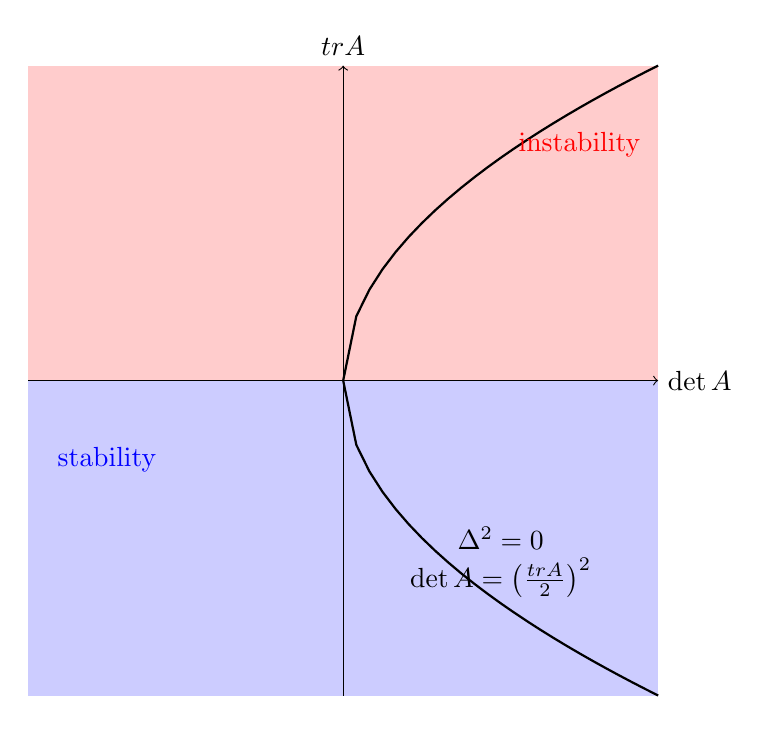
\begin{tikzpicture}
    % Set the size of the grid and the colors
    \fill[red!20] (-4,0) rectangle (4,4);
    \fill[blue!20] (-4,-4) rectangle (4,0);
    
    % Draw the axes
    \draw[->] (-4,0) -- (4,0) node[right] {$\det A$};
    \draw[->] (0,-4) -- (0,4) node[above] {$\operatorname{tr} A$};
    
    % Draw the parabola
    \draw[thick, domain=0:4] plot (\x, {sqrt(\x*4)}) node[right] {};
    \draw[thick, domain=0:4] plot (\x, {-sqrt(\x*4)}) node[right] {};
    
    % Stability and Instability regions
    \node[blue] at (-3,-1) {stability};
    \node[red] at (3,3) {instability};
    
    % Label for the critical point
    \node at (2, -2) {$\Delta^2=0$};
    \node at (2, -2.5) {$\det A = \left(\frac{\operatorname{tr} A}{2}\right)^2$};
\end{tikzpicture}

\citep{murray}


\newpage